% Options for packages loaded elsewhere
\PassOptionsToPackage{unicode}{hyperref}
\PassOptionsToPackage{hyphens}{url}
\PassOptionsToPackage{dvipsnames,svgnames,x11names}{xcolor}
%
\documentclass[
  letterpaper,
  DIV=11,
  numbers=noendperiod]{scrreprt}

\usepackage{amsmath,amssymb}
\usepackage{iftex}
\ifPDFTeX
  \usepackage[T1]{fontenc}
  \usepackage[utf8]{inputenc}
  \usepackage{textcomp} % provide euro and other symbols
\else % if luatex or xetex
  \usepackage{unicode-math}
  \defaultfontfeatures{Scale=MatchLowercase}
  \defaultfontfeatures[\rmfamily]{Ligatures=TeX,Scale=1}
\fi
\usepackage{lmodern}
\ifPDFTeX\else  
    % xetex/luatex font selection
\fi
% Use upquote if available, for straight quotes in verbatim environments
\IfFileExists{upquote.sty}{\usepackage{upquote}}{}
\IfFileExists{microtype.sty}{% use microtype if available
  \usepackage[]{microtype}
  \UseMicrotypeSet[protrusion]{basicmath} % disable protrusion for tt fonts
}{}
\makeatletter
\@ifundefined{KOMAClassName}{% if non-KOMA class
  \IfFileExists{parskip.sty}{%
    \usepackage{parskip}
  }{% else
    \setlength{\parindent}{0pt}
    \setlength{\parskip}{6pt plus 2pt minus 1pt}}
}{% if KOMA class
  \KOMAoptions{parskip=half}}
\makeatother
\usepackage{xcolor}
\setlength{\emergencystretch}{3em} % prevent overfull lines
\setcounter{secnumdepth}{5}
% Make \paragraph and \subparagraph free-standing
\ifx\paragraph\undefined\else
  \let\oldparagraph\paragraph
  \renewcommand{\paragraph}[1]{\oldparagraph{#1}\mbox{}}
\fi
\ifx\subparagraph\undefined\else
  \let\oldsubparagraph\subparagraph
  \renewcommand{\subparagraph}[1]{\oldsubparagraph{#1}\mbox{}}
\fi

\usepackage{color}
\usepackage{fancyvrb}
\newcommand{\VerbBar}{|}
\newcommand{\VERB}{\Verb[commandchars=\\\{\}]}
\DefineVerbatimEnvironment{Highlighting}{Verbatim}{commandchars=\\\{\}}
% Add ',fontsize=\small' for more characters per line
\usepackage{framed}
\definecolor{shadecolor}{RGB}{241,243,245}
\newenvironment{Shaded}{\begin{snugshade}}{\end{snugshade}}
\newcommand{\AlertTok}[1]{\textcolor[rgb]{0.68,0.00,0.00}{#1}}
\newcommand{\AnnotationTok}[1]{\textcolor[rgb]{0.37,0.37,0.37}{#1}}
\newcommand{\AttributeTok}[1]{\textcolor[rgb]{0.40,0.45,0.13}{#1}}
\newcommand{\BaseNTok}[1]{\textcolor[rgb]{0.68,0.00,0.00}{#1}}
\newcommand{\BuiltInTok}[1]{\textcolor[rgb]{0.00,0.23,0.31}{#1}}
\newcommand{\CharTok}[1]{\textcolor[rgb]{0.13,0.47,0.30}{#1}}
\newcommand{\CommentTok}[1]{\textcolor[rgb]{0.37,0.37,0.37}{#1}}
\newcommand{\CommentVarTok}[1]{\textcolor[rgb]{0.37,0.37,0.37}{\textit{#1}}}
\newcommand{\ConstantTok}[1]{\textcolor[rgb]{0.56,0.35,0.01}{#1}}
\newcommand{\ControlFlowTok}[1]{\textcolor[rgb]{0.00,0.23,0.31}{#1}}
\newcommand{\DataTypeTok}[1]{\textcolor[rgb]{0.68,0.00,0.00}{#1}}
\newcommand{\DecValTok}[1]{\textcolor[rgb]{0.68,0.00,0.00}{#1}}
\newcommand{\DocumentationTok}[1]{\textcolor[rgb]{0.37,0.37,0.37}{\textit{#1}}}
\newcommand{\ErrorTok}[1]{\textcolor[rgb]{0.68,0.00,0.00}{#1}}
\newcommand{\ExtensionTok}[1]{\textcolor[rgb]{0.00,0.23,0.31}{#1}}
\newcommand{\FloatTok}[1]{\textcolor[rgb]{0.68,0.00,0.00}{#1}}
\newcommand{\FunctionTok}[1]{\textcolor[rgb]{0.28,0.35,0.67}{#1}}
\newcommand{\ImportTok}[1]{\textcolor[rgb]{0.00,0.46,0.62}{#1}}
\newcommand{\InformationTok}[1]{\textcolor[rgb]{0.37,0.37,0.37}{#1}}
\newcommand{\KeywordTok}[1]{\textcolor[rgb]{0.00,0.23,0.31}{#1}}
\newcommand{\NormalTok}[1]{\textcolor[rgb]{0.00,0.23,0.31}{#1}}
\newcommand{\OperatorTok}[1]{\textcolor[rgb]{0.37,0.37,0.37}{#1}}
\newcommand{\OtherTok}[1]{\textcolor[rgb]{0.00,0.23,0.31}{#1}}
\newcommand{\PreprocessorTok}[1]{\textcolor[rgb]{0.68,0.00,0.00}{#1}}
\newcommand{\RegionMarkerTok}[1]{\textcolor[rgb]{0.00,0.23,0.31}{#1}}
\newcommand{\SpecialCharTok}[1]{\textcolor[rgb]{0.37,0.37,0.37}{#1}}
\newcommand{\SpecialStringTok}[1]{\textcolor[rgb]{0.13,0.47,0.30}{#1}}
\newcommand{\StringTok}[1]{\textcolor[rgb]{0.13,0.47,0.30}{#1}}
\newcommand{\VariableTok}[1]{\textcolor[rgb]{0.07,0.07,0.07}{#1}}
\newcommand{\VerbatimStringTok}[1]{\textcolor[rgb]{0.13,0.47,0.30}{#1}}
\newcommand{\WarningTok}[1]{\textcolor[rgb]{0.37,0.37,0.37}{\textit{#1}}}

\providecommand{\tightlist}{%
  \setlength{\itemsep}{0pt}\setlength{\parskip}{0pt}}\usepackage{longtable,booktabs,array}
\usepackage{calc} % for calculating minipage widths
% Correct order of tables after \paragraph or \subparagraph
\usepackage{etoolbox}
\makeatletter
\patchcmd\longtable{\par}{\if@noskipsec\mbox{}\fi\par}{}{}
\makeatother
% Allow footnotes in longtable head/foot
\IfFileExists{footnotehyper.sty}{\usepackage{footnotehyper}}{\usepackage{footnote}}
\makesavenoteenv{longtable}
\usepackage{graphicx}
\makeatletter
\def\maxwidth{\ifdim\Gin@nat@width>\linewidth\linewidth\else\Gin@nat@width\fi}
\def\maxheight{\ifdim\Gin@nat@height>\textheight\textheight\else\Gin@nat@height\fi}
\makeatother
% Scale images if necessary, so that they will not overflow the page
% margins by default, and it is still possible to overwrite the defaults
% using explicit options in \includegraphics[width, height, ...]{}
\setkeys{Gin}{width=\maxwidth,height=\maxheight,keepaspectratio}
% Set default figure placement to htbp
\makeatletter
\def\fps@figure{htbp}
\makeatother
\newlength{\cslhangindent}
\setlength{\cslhangindent}{1.5em}
\newlength{\csllabelwidth}
\setlength{\csllabelwidth}{3em}
\newlength{\cslentryspacingunit} % times entry-spacing
\setlength{\cslentryspacingunit}{\parskip}
\newenvironment{CSLReferences}[2] % #1 hanging-ident, #2 entry spacing
 {% don't indent paragraphs
  \setlength{\parindent}{0pt}
  % turn on hanging indent if param 1 is 1
  \ifodd #1
  \let\oldpar\par
  \def\par{\hangindent=\cslhangindent\oldpar}
  \fi
  % set entry spacing
  \setlength{\parskip}{#2\cslentryspacingunit}
 }%
 {}
\usepackage{calc}
\newcommand{\CSLBlock}[1]{#1\hfill\break}
\newcommand{\CSLLeftMargin}[1]{\parbox[t]{\csllabelwidth}{#1}}
\newcommand{\CSLRightInline}[1]{\parbox[t]{\linewidth - \csllabelwidth}{#1}\break}
\newcommand{\CSLIndent}[1]{\hspace{\cslhangindent}#1}

\KOMAoption{captions}{tableheading}
\makeatletter
\makeatother
\makeatletter
\@ifpackageloaded{bookmark}{}{\usepackage{bookmark}}
\makeatother
\makeatletter
\@ifpackageloaded{caption}{}{\usepackage{caption}}
\AtBeginDocument{%
\ifdefined\contentsname
  \renewcommand*\contentsname{Table of contents}
\else
  \newcommand\contentsname{Table of contents}
\fi
\ifdefined\listfigurename
  \renewcommand*\listfigurename{List of Figures}
\else
  \newcommand\listfigurename{List of Figures}
\fi
\ifdefined\listtablename
  \renewcommand*\listtablename{List of Tables}
\else
  \newcommand\listtablename{List of Tables}
\fi
\ifdefined\figurename
  \renewcommand*\figurename{Figure}
\else
  \newcommand\figurename{Figure}
\fi
\ifdefined\tablename
  \renewcommand*\tablename{Table}
\else
  \newcommand\tablename{Table}
\fi
}
\@ifpackageloaded{float}{}{\usepackage{float}}
\floatstyle{ruled}
\@ifundefined{c@chapter}{\newfloat{codelisting}{h}{lop}}{\newfloat{codelisting}{h}{lop}[chapter]}
\floatname{codelisting}{Listing}
\newcommand*\listoflistings{\listof{codelisting}{List of Listings}}
\makeatother
\makeatletter
\@ifpackageloaded{caption}{}{\usepackage{caption}}
\@ifpackageloaded{subcaption}{}{\usepackage{subcaption}}
\makeatother
\makeatletter
\@ifpackageloaded{tcolorbox}{}{\usepackage[skins,breakable]{tcolorbox}}
\makeatother
\makeatletter
\@ifundefined{shadecolor}{\definecolor{shadecolor}{rgb}{.97, .97, .97}}
\makeatother
\makeatletter
\makeatother
\makeatletter
\makeatother
\ifLuaTeX
  \usepackage{selnolig}  % disable illegal ligatures
\fi
\IfFileExists{bookmark.sty}{\usepackage{bookmark}}{\usepackage{hyperref}}
\IfFileExists{xurl.sty}{\usepackage{xurl}}{} % add URL line breaks if available
\urlstyle{same} % disable monospaced font for URLs
\hypersetup{
  pdftitle={Wild recipes},
  pdfauthor={Mike Page},
  colorlinks=true,
  linkcolor={blue},
  filecolor={Maroon},
  citecolor={Blue},
  urlcolor={Blue},
  pdfcreator={LaTeX via pandoc}}

\title{Wild recipes}
\author{Mike Page}
\date{2025-10-01}

\begin{document}
\maketitle
\ifdefined\Shaded\renewenvironment{Shaded}{\begin{tcolorbox}[interior hidden, enhanced, borderline west={3pt}{0pt}{shadecolor}, boxrule=0pt, breakable, sharp corners, frame hidden]}{\end{tcolorbox}}\fi

\renewcommand*\contentsname{Table of contents}
{
\hypersetup{linkcolor=}
\setcounter{tocdepth}{2}
\tableofcontents
}
\bookmarksetup{startatroot}

\hypertarget{welcome}{%
\chapter*{Welcome}\label{welcome}}
\addcontentsline{toc}{chapter}{Welcome}

\markboth{Welcome}{Welcome}

The title for this book is inspired by Russ Roberts book, Wild Problems.
In this books he describes a class of problem he calls `wild problems'.
These are big life decisions (e.g., should I move country) where an
algorithmic approach to solving them, such as using a cost-benefit
analysis, often fails. Instead he proposes a new framework to tackle
these problems. (I will leave the curious reader to discover more on
their own)

Much like the `wild problems' discussed in Roberts' book, the R
programmer also faces a class of coding problem which could be described
as wild. That is, a set of problems found outside of a controlled
environment such as a classroom or textbook and instead found in an
environment which is uncontrolled and wild. Here, the examples found
elsewhere often fail, or require a more complex workaround. This could
be due to underlying bugs in R or its libraries, poor documentation, or
quite simply and most often the case, the complexity of the problem
space you are working in doesn't map easily to materials found
elsewhere.

This book is a collection of recipes to some of these wild coding
problems I've experienced in my work as an R programmer. It is by no
means exhausative. Nor is it entriely unique. Indeed, a plethora of
resources already exist in this area and this book even rehashes some of
these (e.g., Stack Overflow, Posit Community, etc.). This book has
primarily been created as a means for myself to document problems I've
faced and the wild recipes I've implemented along the way. My hope is
these recipes might also help you too.

\bookmarksetup{startatroot}

\hypertarget{book-structure}{%
\chapter*{Book structure}\label{book-structure}}
\addcontentsline{toc}{chapter}{Book structure}

\markboth{Book structure}{Book structure}

This book is not designed to be read from cover to cover. Instead it is
written as a collection of individual recipes. Inspired by
\href{https://design.tidyverse.org/}{Tidy design principles}, each
recipe can be read in isolation and will cover:

\begin{itemize}
\item
  What is the problem?
\item
  What is an example?
\item
  What is a solution?
\end{itemize}

Occasionally, recipes will also cover:

\begin{itemize}
\tightlist
\item
  What other solutions exist?
\end{itemize}

\part{ggplot2}

\hypertarget{annotations-text-size}{%
\chapter{Annotations: text size}\label{annotations-text-size}}

\hypertarget{what-is-the-problem}{%
\section{What is the problem?}\label{what-is-the-problem}}

When adding a text annotation to a plot with
\texttt{ggplot2::annotate()}, the size of the text in the annotation
does not match other elements on the plot despite setting the
\texttt{size} argument to equal values.

\hypertarget{what-is-an-example}{%
\section{What is an example?}\label{what-is-an-example}}

\begin{Shaded}
\begin{Highlighting}[]
\FunctionTok{library}\NormalTok{(ggplot2)}

\FunctionTok{ggplot}\NormalTok{() }\SpecialCharTok{+}
  \FunctionTok{ggtitle}\NormalTok{(}\StringTok{"This title is size 14"}\NormalTok{) }\SpecialCharTok{+}
  \FunctionTok{theme}\NormalTok{(}\AttributeTok{plot.title =} \FunctionTok{element\_text}\NormalTok{(}\AttributeTok{size =} \FunctionTok{unit}\NormalTok{(}\DecValTok{14}\NormalTok{, }\StringTok{"pt"}\NormalTok{))) }\SpecialCharTok{+}
  \FunctionTok{annotate}\NormalTok{(}
    \StringTok{"text"}\NormalTok{,}
    \AttributeTok{label =} \StringTok{"This annotation is size 14"}\NormalTok{,}
    \AttributeTok{x =} \DecValTok{0}\NormalTok{, }\AttributeTok{y =} \DecValTok{0}\NormalTok{,}
    \AttributeTok{size =} \FunctionTok{unit}\NormalTok{(}\DecValTok{14}\NormalTok{, }\StringTok{"pt"}\NormalTok{)}
\NormalTok{  )}
\end{Highlighting}
\end{Shaded}

\begin{figure}[H]

{\centering \includegraphics{ggplot2-annotations-sizes_files/figure-pdf/unnamed-chunk-1-1.pdf}

}

\end{figure}

\hypertarget{what-is-a-solution}{%
\section{What is a solution?}\label{what-is-a-solution}}

To align the sizes of annotations and other elements on the plot,
annotation sizes must be divided by \texttt{.pt}:

\begin{Shaded}
\begin{Highlighting}[]
\FunctionTok{ggplot}\NormalTok{() }\SpecialCharTok{+}
  \FunctionTok{ggtitle}\NormalTok{(}\StringTok{"This title is size 14"}\NormalTok{) }\SpecialCharTok{+}
  \FunctionTok{theme}\NormalTok{(}\AttributeTok{plot.title =} \FunctionTok{element\_text}\NormalTok{(}\AttributeTok{size =} \FunctionTok{unit}\NormalTok{(}\DecValTok{14}\NormalTok{, }\StringTok{"pt"}\NormalTok{))) }\SpecialCharTok{+}
  \FunctionTok{annotate}\NormalTok{(}
    \StringTok{"text"}\NormalTok{,}
    \AttributeTok{label =} \StringTok{"This annotation is size 14"}\NormalTok{,}
    \AttributeTok{x =} \DecValTok{0}\NormalTok{, }\AttributeTok{y =} \DecValTok{0}\NormalTok{,}
    \AttributeTok{size =} \FunctionTok{unit}\NormalTok{(}\DecValTok{14}\NormalTok{, }\StringTok{"pt"}\NormalTok{) }\SpecialCharTok{/}\NormalTok{ .pt }\CommentTok{\# divide by .pt}
\NormalTok{  )}
\end{Highlighting}
\end{Shaded}

\begin{figure}[H]

{\centering \includegraphics{ggplot2-annotations-sizes_files/figure-pdf/unnamed-chunk-2-1.pdf}

}

\end{figure}

This works because \texttt{annotate()} calculates font size by
multiplying the specified size by the global variable \texttt{.pt}
(equal to \texttt{2.845276}). See
\href{https://stackoverflow.com/questions/65076492/ggplot-size-of-annotate-vs-size-of-element-text}{this}
Stack Overflow post for more information.

\hypertarget{annotations-infinite-positions}{%
\chapter{Annotations: infinite
positions}\label{annotations-infinite-positions}}

\hypertarget{what-is-the-problem-1}{%
\section{What is the problem?}\label{what-is-the-problem-1}}

To position annotations at the edge of a plot, the values \texttt{Inf}
and \texttt{-Inf} can be passed to the positioning aesthetics (e.g.,
\texttt{x}) of \texttt{ggplot2::annotation()}. This technique fails for
scales that are of class \texttt{Date}.

\hypertarget{what-is-an-example-1}{%
\section{What is an example?}\label{what-is-an-example-1}}

It is useful to first see how we can position annotations on scales
which aren't dates. For example, using the built-in economics dataset of
ggplot2, we can postion an annotation in the top-right corner of the
plot like so:

\begin{Shaded}
\begin{Highlighting}[]
\FunctionTok{library}\NormalTok{(ggplot2)}

\FunctionTok{ggplot}\NormalTok{(economics, }\FunctionTok{aes}\NormalTok{(}\AttributeTok{x =}\NormalTok{ pop, }\AttributeTok{y =}\NormalTok{ unemploy)) }\SpecialCharTok{+}
  \FunctionTok{geom\_point}\NormalTok{() }\SpecialCharTok{+}
  \FunctionTok{annotate}\NormalTok{(}
    \StringTok{"text"}\NormalTok{,}
    \AttributeTok{label =} \StringTok{"Top{-}right"}\NormalTok{,}
    \AttributeTok{vjust =} \DecValTok{1}\NormalTok{, }\AttributeTok{hjust =} \DecValTok{1}\NormalTok{, }\CommentTok{\# Prevent text being chopped}
    \AttributeTok{x =} \ConstantTok{Inf}\NormalTok{, }\AttributeTok{y =} \ConstantTok{Inf}
\NormalTok{  )}
\end{Highlighting}
\end{Shaded}

\begin{figure}[H]

{\centering \includegraphics{ggplot2-annotations-positions_files/figure-pdf/unnamed-chunk-1-1.pdf}

}

\end{figure}

When we try the same approach to a scale that uses dates, we get an
error:

\begin{Shaded}
\begin{Highlighting}[]
\FunctionTok{ggplot}\NormalTok{(economics, }\FunctionTok{aes}\NormalTok{(}\AttributeTok{x =}\NormalTok{ date, }\AttributeTok{y =}\NormalTok{ unemploy)) }\SpecialCharTok{+}
  \FunctionTok{geom\_point}\NormalTok{() }\SpecialCharTok{+}
  \FunctionTok{annotate}\NormalTok{(}
    \StringTok{"text"}\NormalTok{,}
    \AttributeTok{label =} \StringTok{"Top{-}right"}\NormalTok{,}
    \AttributeTok{vjust =} \DecValTok{1}\NormalTok{, }\AttributeTok{hjust =} \DecValTok{1}\NormalTok{, }\CommentTok{\# Prevent text being chopped}
    \AttributeTok{x =} \ConstantTok{Inf}\NormalTok{, }\AttributeTok{y =} \ConstantTok{Inf}
\NormalTok{  )}
\end{Highlighting}
\end{Shaded}

\begin{verbatim}
Error: Invalid input: date_trans works with objects of class Date only
\end{verbatim}

\hypertarget{what-is-a-soltuion}{%
\section{What is a soltuion?}\label{what-is-a-soltuion}}

To plot an annotation at the edge of a scale of class \texttt{Date}, you
should change the class of \texttt{Inf} to a \texttt{Date} class:

\begin{Shaded}
\begin{Highlighting}[]
\FunctionTok{ggplot}\NormalTok{(economics, }\FunctionTok{aes}\NormalTok{(}\AttributeTok{x =}\NormalTok{ date, }\AttributeTok{y =}\NormalTok{ unemploy)) }\SpecialCharTok{+}
  \FunctionTok{geom\_point}\NormalTok{() }\SpecialCharTok{+}
  \FunctionTok{annotate}\NormalTok{(}
    \StringTok{"text"}\NormalTok{,}
    \AttributeTok{label =} \StringTok{"Top{-}right"}\NormalTok{,}
    \AttributeTok{vjust =} \DecValTok{1}\NormalTok{, }\AttributeTok{hjust =} \DecValTok{1}\NormalTok{, }\CommentTok{\# Prevent text being chopped}
    \AttributeTok{x =} \FunctionTok{structure}\NormalTok{(}\ConstantTok{Inf}\NormalTok{, }\AttributeTok{class =} \StringTok{"Date"}\NormalTok{), }\AttributeTok{y =} \ConstantTok{Inf}
\NormalTok{  )}
\end{Highlighting}
\end{Shaded}

\begin{figure}[H]

{\centering 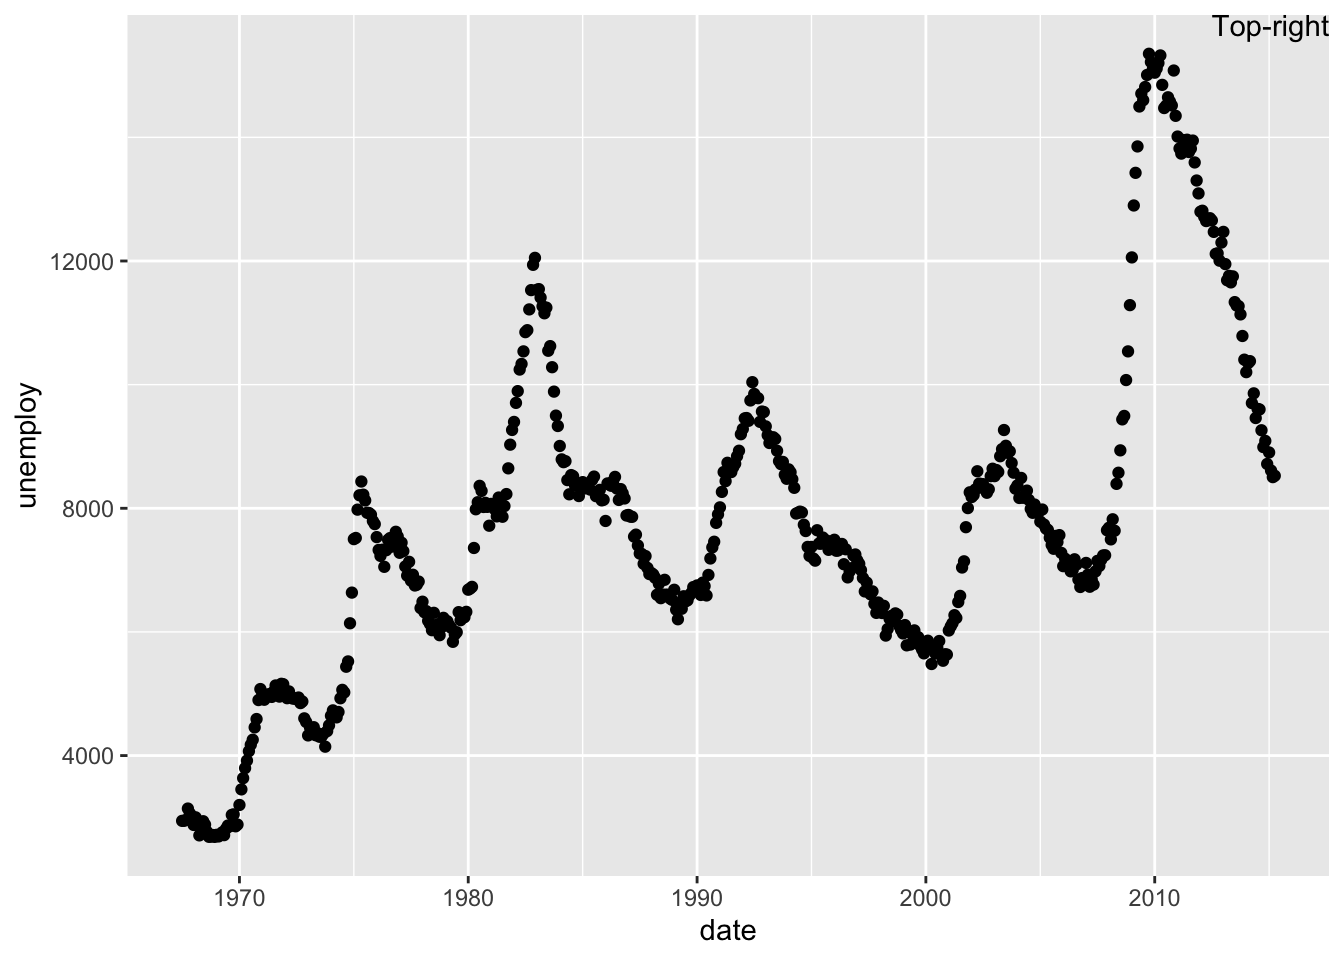
\includegraphics{ggplot2-annotations-positions_files/figure-pdf/unnamed-chunk-3-1.pdf}

}

\end{figure}

See \href{https://github.com/tidyverse/ggplot2/issues/4308}{this} GitHub
issue for more information.

\hypertarget{inspecting-ggplot2-objects}{%
\chapter{Inspecting ggplot2 objects}\label{inspecting-ggplot2-objects}}

\hypertarget{what-is-the-problem-2}{%
\section{What is the problem?}\label{what-is-the-problem-2}}

After creating a ggplot2 object, it can be useful to inspect the object
created, for example, to change the behaviour of functions using that
object, or for writing unit tests. Searching through the
\href{https://ggplot2.tidyverse.org/reference/index.html}{documentation
index} reveals no help, and printing the name of the plot to the console
just calls the default print method, re-printing the plot.

\hypertarget{what-is-an-example-2}{%
\section{What is an example?}\label{what-is-an-example-2}}

Let's create and print a plot with a long subtitle that spans multiple
lines:

\begin{Shaded}
\begin{Highlighting}[]
\FunctionTok{library}\NormalTok{(ggplot2)}

\NormalTok{example }\OtherTok{\textless{}{-}} \FunctionTok{ggplot}\NormalTok{(economics, }\FunctionTok{aes}\NormalTok{(}\AttributeTok{x =}\NormalTok{ pop, }\AttributeTok{y =}\NormalTok{ unemploy)) }\SpecialCharTok{+}
  \FunctionTok{geom\_point}\NormalTok{() }\SpecialCharTok{+}
  \FunctionTok{labs}\NormalTok{(}
    \AttributeTok{title =} \StringTok{"Title"}\NormalTok{,}
    \AttributeTok{subtitle =} \FunctionTok{paste0}\NormalTok{(}
      \StringTok{"This is a long subtitle that spans multiple lines and serves as a nice demonstratation for this"}\NormalTok{,}
      \StringTok{"}\SpecialCharTok{\textbackslash{}n}\StringTok{"}\NormalTok{,}
      \StringTok{"example about inspecting ggplot objects"}
\NormalTok{    )}
\NormalTok{  )}

\NormalTok{example}
\end{Highlighting}
\end{Shaded}

\begin{figure}[H]

{\centering \includegraphics{ggplot2-objects_files/figure-pdf/unnamed-chunk-1-1.pdf}

}

\end{figure}

Now, we want to write a wrapper function to \texttt{ggsave()} that
changes the \texttt{height} parameter of the output plot, depending on
whether a multiline subtitle has been detected.

\hypertarget{what-is-a-solution-1}{%
\section{What is a solution?}\label{what-is-a-solution-1}}

Internally, a ggplot object is just stored as a list, and can be
inspected with \texttt{str()} like most objects:

\begin{Shaded}
\begin{Highlighting}[]
\FunctionTok{typeof}\NormalTok{(example)}
\end{Highlighting}
\end{Shaded}

\begin{verbatim}
[1] "list"
\end{verbatim}

\begin{Shaded}
\begin{Highlighting}[]
\FunctionTok{str}\NormalTok{(example)}
\end{Highlighting}
\end{Shaded}

\begin{verbatim}
List of 9
 $ data       : spc_tbl_ [574 x 6] (S3: spec_tbl_df/tbl_df/tbl/data.frame)
  ..$ date    : Date[1:574], format: "1967-07-01" "1967-08-01" ...
  ..$ pce     : num [1:574] 507 510 516 512 517 ...
  ..$ pop     : num [1:574] 198712 198911 199113 199311 199498 ...
  ..$ psavert : num [1:574] 12.6 12.6 11.9 12.9 12.8 11.8 11.7 12.3 11.7 12.3 ...
  ..$ uempmed : num [1:574] 4.5 4.7 4.6 4.9 4.7 4.8 5.1 4.5 4.1 4.6 ...
  ..$ unemploy: num [1:574] 2944 2945 2958 3143 3066 ...
 $ layers     :List of 1
  ..$ :Classes 'LayerInstance', 'Layer', 'ggproto', 'gg' <ggproto object: Class LayerInstance, Layer, gg>
    aes_params: list
    compute_aesthetics: function
    compute_geom_1: function
    compute_geom_2: function
    compute_position: function
    compute_statistic: function
    computed_geom_params: list
    computed_mapping: uneval
    computed_stat_params: list
    constructor: call
    data: waiver
    draw_geom: function
    finish_statistics: function
    geom: <ggproto object: Class GeomPoint, Geom, gg>
        aesthetics: function
        default_aes: uneval
        draw_group: function
        draw_key: function
        draw_layer: function
        draw_panel: function
        extra_params: na.rm
        handle_na: function
        non_missing_aes: size shape colour
        optional_aes: 
        parameters: function
        rename_size: FALSE
        required_aes: x y
        setup_data: function
        setup_params: function
        use_defaults: function
        super:  <ggproto object: Class Geom, gg>
    geom_params: list
    inherit.aes: TRUE
    layer_data: function
    map_statistic: function
    mapping: NULL
    position: <ggproto object: Class PositionIdentity, Position, gg>
        compute_layer: function
        compute_panel: function
        required_aes: 
        setup_data: function
        setup_params: function
        super:  <ggproto object: Class Position, gg>
    print: function
    setup_layer: function
    show.legend: NA
    stat: <ggproto object: Class StatIdentity, Stat, gg>
        aesthetics: function
        compute_group: function
        compute_layer: function
        compute_panel: function
        default_aes: uneval
        dropped_aes: 
        extra_params: na.rm
        finish_layer: function
        non_missing_aes: 
        optional_aes: 
        parameters: function
        required_aes: 
        retransform: TRUE
        setup_data: function
        setup_params: function
        super:  <ggproto object: Class Stat, gg>
    stat_params: list
    super:  <ggproto object: Class Layer, gg> 
 $ scales     :Classes 'ScalesList', 'ggproto', 'gg' <ggproto object: Class ScalesList, gg>
    add: function
    clone: function
    find: function
    get_scales: function
    has_scale: function
    input: function
    n: function
    non_position_scales: function
    scales: list
    super:  <ggproto object: Class ScalesList, gg> 
 $ mapping    :List of 2
  ..$ x: language ~pop
  .. ..- attr(*, ".Environment")=<environment: R_GlobalEnv> 
  ..$ y: language ~unemploy
  .. ..- attr(*, ".Environment")=<environment: R_GlobalEnv> 
  ..- attr(*, "class")= chr "uneval"
 $ theme      : list()
 $ coordinates:Classes 'CoordCartesian', 'Coord', 'ggproto', 'gg' <ggproto object: Class CoordCartesian, Coord, gg>
    aspect: function
    backtransform_range: function
    clip: on
    default: TRUE
    distance: function
    expand: TRUE
    is_free: function
    is_linear: function
    labels: function
    limits: list
    modify_scales: function
    range: function
    render_axis_h: function
    render_axis_v: function
    render_bg: function
    render_fg: function
    setup_data: function
    setup_layout: function
    setup_panel_guides: function
    setup_panel_params: function
    setup_params: function
    train_panel_guides: function
    transform: function
    super:  <ggproto object: Class CoordCartesian, Coord, gg> 
 $ facet      :Classes 'FacetNull', 'Facet', 'ggproto', 'gg' <ggproto object: Class FacetNull, Facet, gg>
    compute_layout: function
    draw_back: function
    draw_front: function
    draw_labels: function
    draw_panels: function
    finish_data: function
    init_scales: function
    map_data: function
    params: list
    setup_data: function
    setup_params: function
    shrink: TRUE
    train_scales: function
    vars: function
    super:  <ggproto object: Class FacetNull, Facet, gg> 
 $ plot_env   :<environment: R_GlobalEnv> 
 $ labels     :List of 4
  ..$ title   : chr "Title"
  ..$ subtitle: chr "This is a long subtitle that spans multiple lines and serves as a nice demonstratation for this\nexample about "| __truncated__
  ..$ x       : chr "pop"
  ..$ y       : chr "unemploy"
 - attr(*, "class")= chr [1:2] "gg" "ggplot"
\end{verbatim}

Here, we can see and access all the elements that make up the plot
(e.g., scales, data, etc.). The subtitle can be accessed like so:

\begin{Shaded}
\begin{Highlighting}[]
\NormalTok{subtitle }\OtherTok{\textless{}{-}}\NormalTok{ example}\SpecialCharTok{$}\NormalTok{labels}\SpecialCharTok{$}\NormalTok{subtitle}
\end{Highlighting}
\end{Shaded}

We could then write a wrapper function to detect whether our subtitle is
multiline and change the \texttt{height} of \texttt{ggsave()}
accordingly:

\begin{Shaded}
\begin{Highlighting}[]
\NormalTok{ggsave\_multline }\OtherTok{\textless{}{-}} \ControlFlowTok{function}\NormalTok{(...) \{}
\NormalTok{  height }\OtherTok{\textless{}{-}} \FunctionTok{ifelse}\NormalTok{(}\FunctionTok{grepl}\NormalTok{(}\StringTok{"}\SpecialCharTok{\textbackslash{}\textbackslash{}}\StringTok{n"}\NormalTok{, subtitle), }\DecValTok{11}\NormalTok{, }\DecValTok{10}\NormalTok{)}
  \FunctionTok{ggsave}\NormalTok{(}\AttributeTok{height =}\NormalTok{ height, ...)}
\NormalTok{\}}
\end{Highlighting}
\end{Shaded}

\hypertarget{what-other-solutions-exist}{%
\section{What other solutions exist?}\label{what-other-solutions-exist}}

ggplot2 provides a set of
\href{https://ggplot2.tidyverse.org/reference/ggplot_build.html}{functions}
to render plot objects, which can also be used to inspect the underlying
data and panel object. These functions
\href{https://github.com/tidyverse/ggplot2/blob/HEAD/R/plot-build.R\#L21}{do
not appear} in the documentation index however, and so are not easily
discoverable. For a deeper diver on these functions and the internals of
ggplot objects, see \href{https://ggplot2-book.org/internals}{this
chapter} in the book ``ggplot2: Elegant Graphics for Data Analysis
(3e)''.

\hypertarget{panel-sizes}{%
\chapter{Panel sizes}\label{panel-sizes}}

\hypertarget{what-is-the-problem-3}{%
\section{What is the problem?}\label{what-is-the-problem-3}}

There is no default method to set the panel size of a plot in ggplot2,
only a method to set the plot size using the \texttt{width} and
\texttt{height} paramaeters of \texttt{ggplot2::ggsave()}. The panel
refers to the inner plotting window that contains the data, and the plot
refers to the whole plotting window that contains both the panel and all
other elements (e.g., legeneds, labels, etc.):

\includegraphics{ggplot2-panel-sizes_files/figure-pdf/unnamed-chunk-1-1.pdf}

\hypertarget{what-is-a-solution-2}{%
\section{What is a solution?}\label{what-is-a-solution-2}}

The
\href{https://teunbrand.github.io/ggh4x/reference/force_panelsizes.html}{\texttt{ggh4x::force\_panelsizes()}}
function can be used to coerce a single panel to a set size:

\begin{Shaded}
\begin{Highlighting}[]
\FunctionTok{library}\NormalTok{(ggplot2)}

\FunctionTok{ggplot}\NormalTok{(economics, }\FunctionTok{aes}\NormalTok{(}\AttributeTok{x =}\NormalTok{ pop, }\AttributeTok{y =}\NormalTok{ unemploy)) }\SpecialCharTok{+}
  \FunctionTok{geom\_point}\NormalTok{() }\SpecialCharTok{+}
\NormalTok{  ggh4x}\SpecialCharTok{::}\FunctionTok{force\_panelsizes}\NormalTok{(}
    \AttributeTok{rows =} \FunctionTok{unit}\NormalTok{(}\DecValTok{8}\NormalTok{, }\StringTok{"cm"}\NormalTok{),}
    \AttributeTok{cols =} \FunctionTok{unit}\NormalTok{(}\DecValTok{12}\NormalTok{, }\StringTok{"cm"}\NormalTok{)}
\NormalTok{  )}
\end{Highlighting}
\end{Shaded}

\begin{figure}[H]

{\centering \includegraphics{ggplot2-panel-sizes_files/figure-pdf/unnamed-chunk-2-1.pdf}

}

\end{figure}

\bookmarksetup{startatroot}

\hypertarget{references}{%
\chapter*{References}\label{references}}
\addcontentsline{toc}{chapter}{References}

\markboth{References}{References}

\hypertarget{refs}{}
\begin{CSLReferences}{0}{0}
\end{CSLReferences}



\end{document}
